\documentclass[12pt]{article}
\usepackage{amsmath}
\usepackage{amssymb}
\usepackage[letterpaper,margin=0.85in,centering]{geometry}
\usepackage{fancyhdr}
\usepackage{enumerate}
\usepackage{lastpage}
\usepackage{multicol}
\usepackage{graphicx}
\usepackage{tikz}
\usetikzlibrary{calc, positioning, decorations.pathmorphing}


\reversemarginpar

\pagestyle{fancy}
\cfoot{}
\lhead{Math 1560}\chead{Tutorial Assignment \# 7 Solutions}\rhead{June 1st, 2017}
%\rfoot{Total: 10 points}
%\chead{{\bf Name:}}
\newcommand{\points}[1]{\marginpar{\hspace{24pt}[#1]}}
\newcommand{\skipline}{\vspace{12pt}}
%\renewcommand{\headrulewidth}{0in}
\headheight 30pt

\newcommand{\di}{\displaystyle}
\newcommand{\abs}[1]{\lvert #1\rvert}
\newcommand{\len}[1]{\lVert #1\rVert}
\renewcommand{\i}{\mathbf{i}}
\renewcommand{\j}{\mathbf{j}}
\renewcommand{\k}{\mathbf{k}}
\newcommand{\R}{\mathbb{R}}
\newcommand{\aaa}{\mathbf{a}}
\newcommand{\bbb}{\mathbf{b}}
\newcommand{\ccc}{\mathbf{c}}
\newcommand{\dotp}{\boldsymbol{\cdot}}
\newcommand{\bbm}{\begin{bmatrix}}
\newcommand{\ebm}{\end{bmatrix}}                   
                  
\begin{document}

%\author{Instructor: Sean Fitzpatrick}
\thispagestyle{fancy}
%\noindent{{\bf Name and student number:}}

 \begin{enumerate}
  \item Sketch the graph of $f(x) = \dfrac{x}{x^2-2x+1}$. Your solution should include the following:
\begin{itemize}
 \item The domain of $f$, and all intercepts and asymptotes.
 \item The critical points of $f$, including the location of any local maxima or minima.
 \item The intervals on which $f$ is increasing or decreasing.
 \item The inflection points of $f$, and the intervals on which $f$ is concave up or concave down.
\end{itemize}

\bigskip

Since $f(x) = \frac{x}{(x-1)^2}$, we see that there is a vertical asymptote at $x=1$, and $f(0)=0$ is the only $x$-intercept (which happens to also be the $y$-intercept). The sign diagram for $f$ is given by
\begin{center}
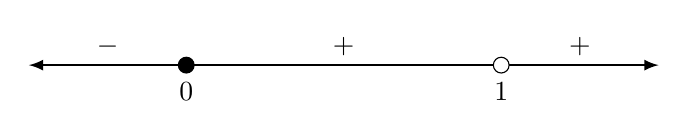
\begin{tikzpicture}[>=latex]
  \draw [thick, <->] (-4,0) -- (4,0);
  \draw [fill] (-2,0) circle [radius =.1];
  \draw [fill=white] (2,0) circle [radius =.1];
  \node at (-3,0) [above] {$-$};
  \node at (0,0) [above] {$+$};
  \node at (3,0) [above] {$+$};
  \node at (-2,-0.1) [below] {$0$};
  \node at (2,-0.1) [below] {$1$};
  \end{tikzpicture}
\end{center}

The first derivative of $f$ is
\[
 f'(x) = \frac{(1)(x-1)^2-x(2)(x-1)}{((x-1)^2)^2} = \frac{(x-1)((x-1)-2x)}{(x-1)^4} = \frac{-(x+1)}{(x-1)^3}.
\]
We see that $f'(-1)=0$, so $x=-1$ is the only critical point. (Note $x=1$ is not in the domain of $f$. The sign diagram for $f'$ is given by
\begin{center}
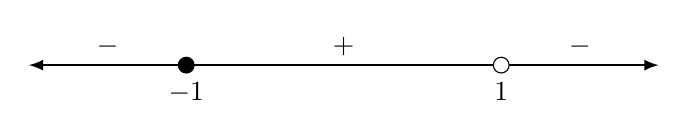
\begin{tikzpicture}[>=latex]
  \draw [thick, <->] (-4,0) -- (4,0);
  \draw [fill] (-2,0) circle [radius =.1];
  \draw [fill=white] (2,0) circle [radius =.1];
  \node at (-3,0) [above] {$-$};
  \node at (0,0) [above] {$+$};
  \node at (3,0) [above] {$-$};
  \node at (-2,-0.1) [below] {$-1$};
  \node at (2,-0.1) [below] {$1$};
  \end{tikzpicture}
\end{center}
From the sign diagram, we see that $(-1,f(-1))=(-1,-1/4)$ is a local minimum, and that $f$ is increasing on $(-1,1)$, and decreasing on $(-\infty, -1)\cup (1,\infty)$.

The second derivative of $f$ is
\[
 f''(x) = \frac{d}{dx}\left(\frac{-(x+1)}{(x-1)^3}\right) = -\frac{(x-1)^3-(x+1)(3(x-1)^2)}{(x-1)^6} = -\frac{(x-1)-3(x+1)}{(x-1)^4} = \frac{2(x+2)}{(x-1)^4}.
\]
We see that $f''(-2)=0$, and this is the only possible inflection point. The sign diagram for $f''$ is given by
\begin{center}
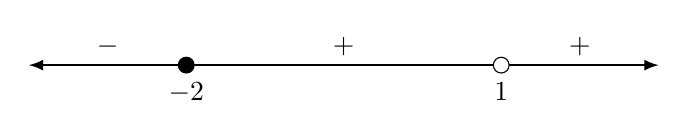
\begin{tikzpicture}[>=latex]
  \draw [thick, <->] (-4,0) -- (4,0);
  \draw [fill] (-2,0) circle [radius =.1];
  \draw [fill=white] (2,0) circle [radius =.1];
  \node at (-3,0) [above] {$-$};
  \node at (0,0) [above] {$+$};
  \node at (3,0) [above] {$+$};
  \node at (-2,-0.1) [below] {$-2$};
  \node at (2,-0.1) [below] {$1$};
  \end{tikzpicture}
\end{center}
We see that $(-2,f(-2))=(-2,-2/9)$ is an inflection point, and that the graph of $f$ is concave up on $(-2,1)\cup (1,\infty)$, and concave down on $(-\infty,-2)$.

The graph of $f$ is given below:
\begin{center}
 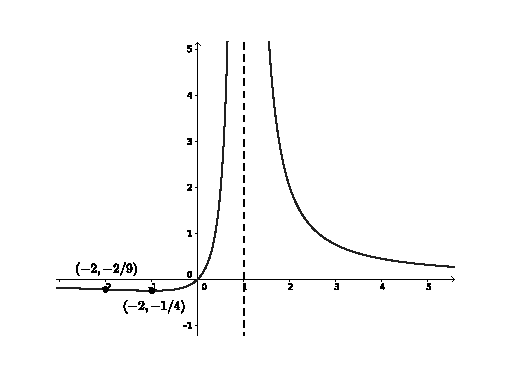
\includegraphics[width=5in]{WS7-graph}
\end{center}


\item At noon, ship A (`The Valiant') is 100 km west of ship B ('Excelsior'). Ship A is sailing south at 35 km/h, and ship B is steaming north at 25 km/h. How fast is the distance between the ships changing at 4:00 pm?

\bigskip

\begin{multicols}{2}
 A diagram of the situation is shown to the right. After $t$ hours, Ship A will be $35t$ km south of its original position, and Ship $B$ will be $25t$ km north of its original position. The distance $z$ between the ships is the length of the hypotenuse of the large right-angled triangle with base length 100 km, and height given by $35t+25t=60t$. The distance between the ships therefore satisfies the equation
\[
 z^2 = 100^2+(60t)^2.
\]
 \columnbreak
 \begin{center}
  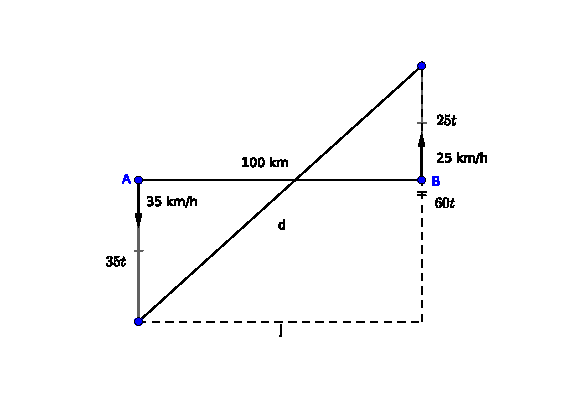
\includegraphics[width=0.9\columnwidth]{WS7-2sol}
 \end{center}

\end{multicols}
Differentiating both sides of the equation $z^2=10000+3600t^2$ with respect to $t$, we obtain:
\[
 2z\frac{dz}{dt} = 7200t,
\]
so $\dfrac{dz}{dt} = \dfrac{3600t}{z}$. At 4:00 pm, we have $t=4$, and $z^2 = 10000+(3600)(4^2)=67600=260^2$. Thus, we find
\[
 \dfrac{dz}{dt} = \frac{3600(4)}{260} \approx 55.4 \text{ km/h}.
\]

\bigskip

\item An 8-foot-tall fence runs parallel to a tall building, at a distance of 4 feet from the building. What is the length of the shortest ladder that will reach from the ground, over the fence, to the wall of the building?

\bigskip

\begin{multicols}{2}
 The diagram to the right shows our piece of cardboard, and the squares to be removed. The volume of our box is given by $V=l\cdot w\cdot h$, where $l$ is the length, $w$ is the width, and $h$ is the height. We immediately see that $h=x$, while the length and width are each obtained by subtracting $2x$ (the amount being cut out) from the original length and width of the cardboard. Therefore, we have $l=15-2x$, and $w=8-2x$.
 \columnbreak
 \begin{center}
  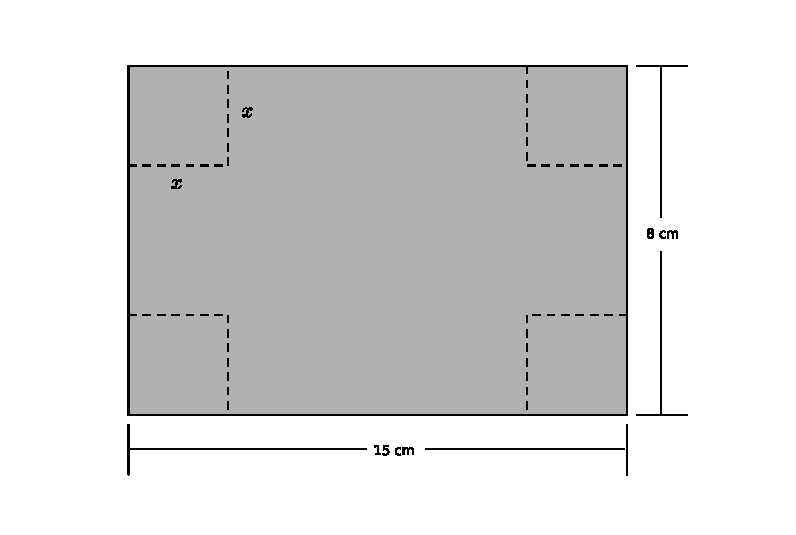
\includegraphics[width=0.9\columnwidth]{WS7-3sol}
 \end{center}

\end{multicols}
The volume of the box is therefore
\[
 V(x) = x(15-2x)(8-2x) = 120x-46x^2+4x^3.
\]
We note that we must have $0\leq x\leq 4$, since $x$ cannot be negative (it's a length), and it cannot be more than half the width. As we might expect, $V(0)=0$ and $V(4)=0$, so the maximum volume will be obtained at some critical point, where $V'(x)=0$. We find
\[
 V'(x) = 120-92x+12x^2,
\]
and with the help of a calculator, we find that $V'(x)=0$ for $x=6$ or $x=5/3$. Since $x=6$ is outside the domain for $V$, we must have $x=5/3$. We can quickly check that $V''(x)=24x-92$, so $V''(5/3) = 40-92=-52<0$, telling us that the critical point at $x=5/3$ is, indeed, a maximum.

Thus, we should remove squares of length $5/3$ cm from each corner.
\end{enumerate}

\end{document}